\chapter{Movement}\label{ch:move}
For our robot to be able to show the results of path finding,
it needed to be able to move.

We decided to move only along a simple 2D grid-like structure,
therefore wheels were the easiest solution.
\section{Motors}\label{sec:motors}
A stepper motor is a motor that moves one step at a time, with its step defined by a step angle.

\begin{figure}[h]
	\centering
	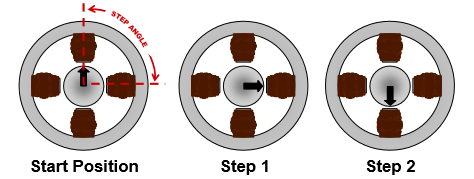
\includegraphics[width=\textwidth]{figures/move/motor1.png}
	\caption{Step Angle}
\end{figure}

The image above represents a stepper motor that requires 4 steps to complete a 360 degrees rotation. This determines the step angle to be 90 degrees. 
The main components of a stepper motor are represented in the image below, and they consist of stators, windings(phases), and rotor.
The part that moves, is the rotor, which can be magnetized or not, depending on the type of stepper motor.

\begin{figure}[h]
	\centering
	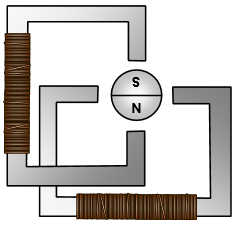
\includegraphics[width=0.5\textwidth]{figures/move/motor2.png}
	\caption{Main Components}
\end{figure}

By applying a voltage across one of the windings, current will start flowing through it. By using the right-hand rule, the direction of the magnetic flux can be determined. This is represented in the image below.

\begin{figure}[h]
	\centering
	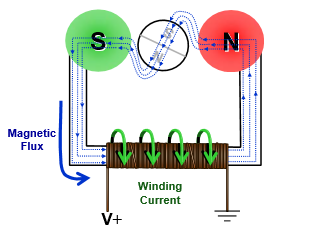
\includegraphics[width=0.6\textwidth]{figures/move/motor3.png}
	\caption{Direction of Magnetic Flux}
\end{figure}

The flux will want to travel through the path that has the least resistance. This determines the rotor to change its position to minimize resistance. This is shown in the image below.

\begin{figure}[h]
	\centering
	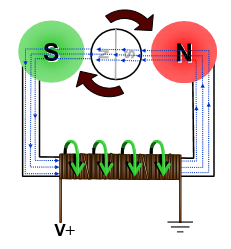
\includegraphics[width=0.5\textwidth]{figures/move/motor4.png}
	\caption{Direction of Magnetic Flux 2}
\end{figure}
\subsection{Types of Stepper Motors}
\subsubsection{Permanent Magnet Motor}
This type of stepper motor has a magnetized rotor. Each winding, will be subdivided into two, to better understand how to motor functions. The image below represents the windings, and how they are distributed inside a stepper motor.

\begin{figure}[htp] 
    \centering
    \subfloat[Rotor]{%
        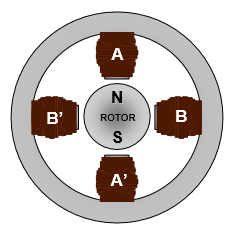
\includegraphics[width=0.4\textwidth]{figures/move/motor5.png}%
        }%
    \hfill%
    \subfloat[Winding]{%
        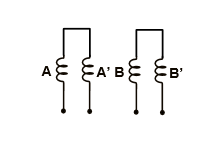
\includegraphics[width=0.4\textwidth]{figures/move/motor6.png}%
        }%
\end{figure}

The resolution of the motor can be improved in two ways, either by increasing the number of pole pairs in the rotor itself, or by increasing the number of phases as shown below.


\begin{figure}[htp] 
    \centering
    \subfloat[Increased Pole Pairs]{%
        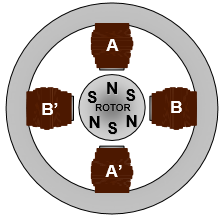
\includegraphics[width=0.4\textwidth]{figures/move/motor7.png}%
        }%
    \hfill%
    \subfloat[Increased Number of Winding]{%
        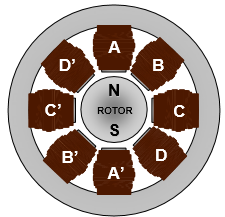
\includegraphics[width=0.4\textwidth]{figures/move/motor8.png}%
        }%
\end{figure}

To rotate the motor, simply apply a voltage across the windings in a sequence. A full rotation is shown in the images below, with the corresponding phase energized.

\begin{figure}[htp] 
    \centering
    \subfloat[$1\textsuperscript{st}$ Step]{
        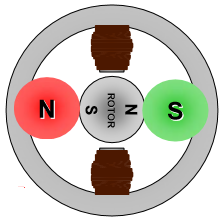
\includegraphics[width=0.2\textwidth]{figures/move/motor9.png}
        }
    \hfill
    \subfloat[$2\textsuperscript{nd}$ Step]{
        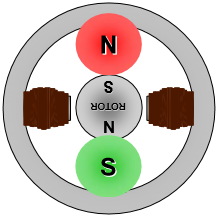
\includegraphics[width=0.2\textwidth]{figures/move/motor10.png}
        }
    \hfill
    \subfloat[$3\textsuperscript{rd}$ Step]{
    	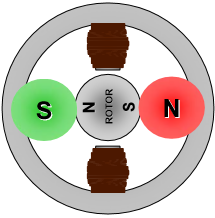
\includegraphics[width=0.2\textwidth]{figures/move/motor11.png}
    	}
  	\hfill
  	\subfloat[$4\textsuperscript{th}$ Step]{
  		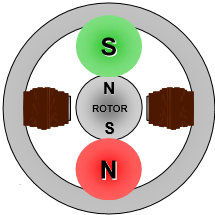
\includegraphics[width=0.2\textwidth]{figures/move/motor12.png}
  		}
\end{figure}

\begin{figure}[htp] 
    \centering
    \subfloat[$1\textsuperscript{st}$ Step Winding]{
        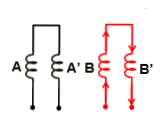
\includegraphics[width=0.2\textwidth]{figures/move/motor13.png}
        }
    \hfill
    \subfloat[$2\textsuperscript{nd}$ Step Winding]{
        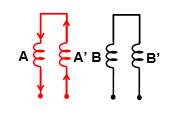
\includegraphics[width=0.2\textwidth]{figures/move/motor14.png}
        }
    \hfill
    \subfloat[$3\textsuperscript{rd}$ Step Winding]{
    	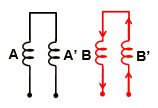
\includegraphics[width=0.2\textwidth]{figures/move/motor15.png}
    	}
  	\hfill
  	\subfloat[$4\textsuperscript{th}$ Winding]{
  		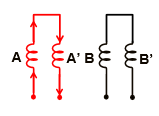
\includegraphics[width=0.2\textwidth]{figures/move/motor16.png}
  		}
\end{figure}
\subsubsection{Variable Reluctance Motor}
This type of motor, uses a rotor that is not magnetized, and has a number of teeth as seen in the image below. The windings are configured differently, as depicted in the second figure, all having a common voltage source but with each end being separate. They usually have 3 or 5 windings. Greater precision can be achieved by adding more teeth to the rotor.

\begin{figure}[htp] 
    \centering
    \subfloat[Non Magnetized Rotor]{
        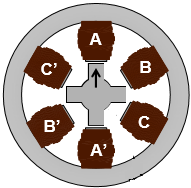
\includegraphics[width=0.4\textwidth]{figures/move/motor17.png}
        }
    \hfill
    \subfloat[Windings]{%
        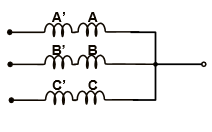
\includegraphics[width=0.4\textwidth]{figures/move/motor18.png}
        }
\end{figure}

To spin the motor, each winding is energized one at a time, and the rotor rotates in such a way, to minimize reluctance. Some of the differences, between this type of stepper motor and the permanent magnet motor, are that, in order to spin the motor in a direction, the windings have to be energized in a reverse sequence, as depicted in the images below. In addition, the step angle is actually half of the one of a permanent magnet motor with the same number of windings is.

\begin{figure}[htp] 
    \centering
    \subfloat[$1\textsuperscript{st}$ Step]{
        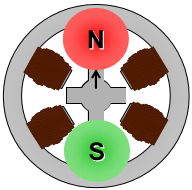
\includegraphics[width=0.2\textwidth]{figures/move/motor19.png}
        }
    \hfill
    \subfloat[$2\textsuperscript{nd}$ Step]{
        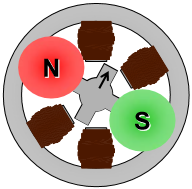
\includegraphics[width=0.2\textwidth]{figures/move/motor20.png}
        }
    \hfill
    \subfloat[$3\textsuperscript{rd}$ Step]{
    	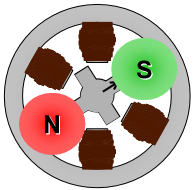
\includegraphics[width=0.2\textwidth]{figures/move/motor21.png}
    	}
  	\hfill
  	\subfloat[$4\textsuperscript{th}$ Step]{
  		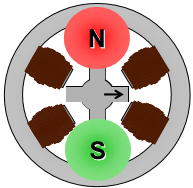
\includegraphics[width=0.2\textwidth]{figures/move/motor22.png}
  		}
\end{figure}

\begin{figure}[htp] 
    \centering
    \subfloat[$1\textsuperscript{st}$ Step Winding]{
        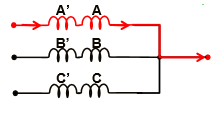
\includegraphics[width=0.2\textwidth]{figures/move/motor23.png}
        }
    \hfill
    \subfloat[$2\textsuperscript{nd}$ Step Winding]{
        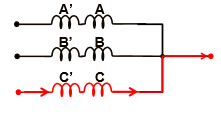
\includegraphics[width=0.2\textwidth]{figures/move/motor24.png}
        }
    \hfill
    \subfloat[$3\textsuperscript{rd}$ Step Winding]{
    	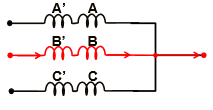
\includegraphics[width=0.2\textwidth]{figures/move/motor25.png}
    	}
  	\hfill
  	\subfloat[$4\textsuperscript{th}$ Winding]{
  		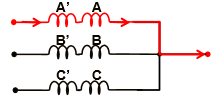
\includegraphics[width=0.2\textwidth]{figures/move/motor26.png}
  		}
\end{figure}

\subsubsection{Hybrid Stepper Motor}
Hybrid stepper motors borrow characteristics both the previous ones. The picture below shows the two of the main components of the hybrid stepper motor. On the left side, the stator can be seen consisting of 8 poles. On the right side, is represented the rotor. The rotor consists of two sets of teeth, corresponding for the two poles, north and south, respectively.

\begin{figure}[h]
	\centering
	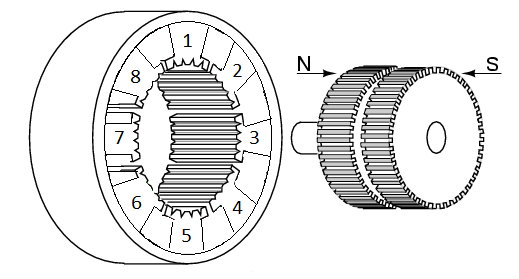
\includegraphics[width=\textwidth]{figures/move/motor27.png}
	\caption{Stator And Rotor}
\end{figure}

It is important to notice two additional things. The first, is that the teeth on the rotor are not aligned but are interleaved, as shown in the picture below. The second, is the placement of the stator teeth in respect to those of the rotor, represented in the second picture.

\begin{figure}[htp] 
    \centering
    \subfloat[Interleaved Teeth]{
        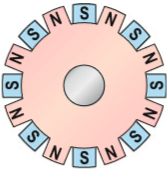
\includegraphics[width=0.4\textwidth]{figures/move/motor28.png}
        }
    \hfill
    \subfloat[Stepper Motor Inside]{%
        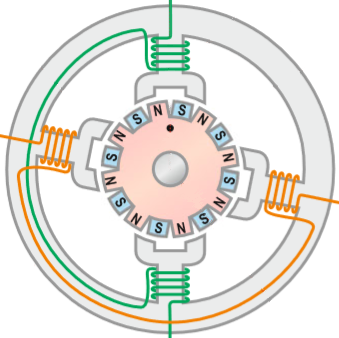
\includegraphics[width=0.4\textwidth]{figures/move/motor29.png}
        }
\end{figure}

It can be observed in the second picture, the windings with numbers 1 and 5 are completely aligned with the teeth of the rotor. Windings number 3 and 7 are completely unaligned, while the others are half aligned. This results in higher precision and higher torque offered by the hybrid stepper motor, depending on the stepping method used.

The picture below represents the front view of the hybrid stepper motor together with the configuration of the two windings. 

\begin{figure}[htp] 
    \centering
    \subfloat[Front View Stepper Motor]{
        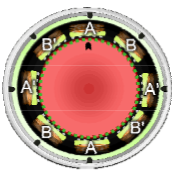
\includegraphics[width=0.4\textwidth]{figures/move/motor30.png}
        }
    \hfill
    \subfloat[Winding Configuration]{%
        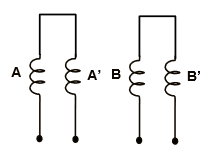
\includegraphics[width=0.4\textwidth]{figures/move/motor31.png}
        }
\end{figure}

It is important to notice that, even though the motor has only two windings, each individual winding energizes 4 stator poles.

\section{Motor Drivers}\label{sec:drivers}
\section{Wheels}\label{sec:wheels}
We wanted the robot to be capable of moving in eight directions from every position.
One solution for this would have been for the robot to turn every time it needed to change direction,
but since our goal was to test and time our path finding algorithm,
this was highly impractical.
One of our group members had worked with small wheel-based robots before,
and remembered omni-wheels.
\begin{figure}[htp]
	\centering
	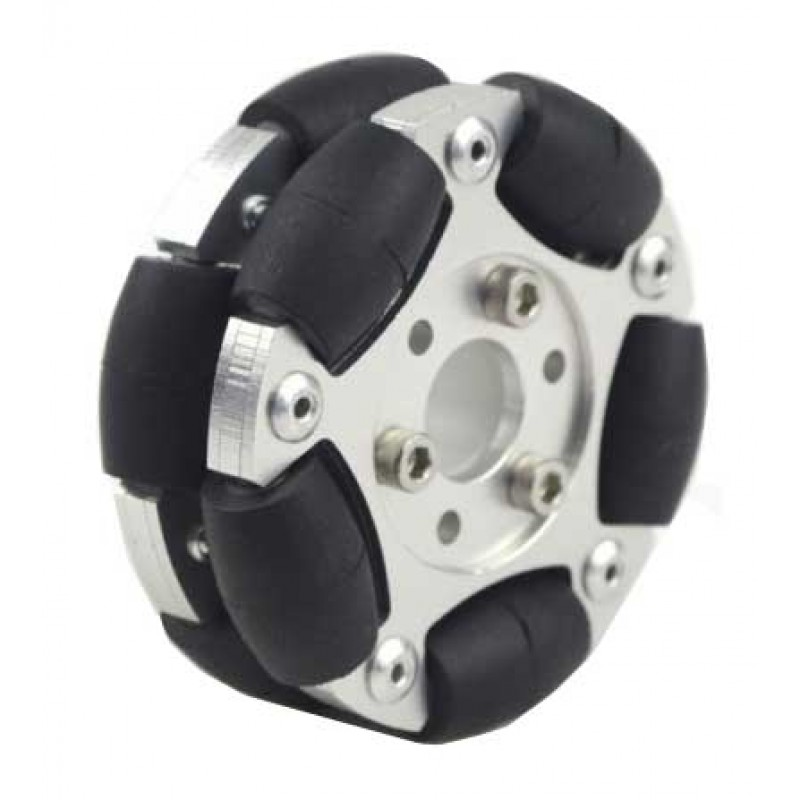
\includegraphics[width=0.2\textwidth]{figures/move/omni_wheel}
	\caption{motor control circuit}
	\label{fig:omni}
\end{figure}
Omni-wheels are wheels,
whose contact area consists of smaller wheels.
Those smaller wheels are able to spin freely,
with very little force needed.
If mounted in two pairs,
with the axes crossing at a 90 degree angle, \todo{find degree symbol}
one pair controls all forces along the x-axis,
and the other one along the y-axis.
\missingfigure{a figure of the forces in different directions added together}

\section{Direction Control}\label{sec:direction}
To control the direction of the robot,
we had to control which wheels turn how many degrees.

One option for this would have been to control each motor individually,
for this we would have needed four individually controllable stepper motors,
and four times four control outputs from our microcontroller.
This solution also meant precise timing between the four motors was needed,
in order to not generate any rotation.

We decided to look for a solution using less output pins,
and without the danger of rotation.

By analysing the requirements for our directional control,
we figured out that we only need 8 configurations of motor pairs.
\begin{center}
\begin{tabular}{|l|l|l|}
	\hline
	Direction & Pair A & Pair B	\\
	\hline
	North & forward & forward \\
	East 	& forward & backward \\
	South & backward & backward \\
	West 	& backward & forward \\
	\hline
	North-East & forward & off \\
	South-East & off & backward \\
	South-West & backward & off\\
	North-West & off & forward \\
	\hline
\end{tabular}
\begin{tabular}{|l|c|c|c|c|}
	\hline
	Direction & Aflip & Aon & Bflip & Bon \\
	\hline
	North & 0 & 1 & 0 & 1 \\
	East 	& 0 & 1 & 1 & 1 \\
	South & 1 & 1 & 1 & 1 \\
	West 	& 1 & 1 & 0 & 1 \\
	\hline
	North-East & 0 & 1 & 1 & 0 \\
	South-East & 1 & 0 & 0 & 1 \\
	South-West & 1 & 1 & 1 & 0 \\
	North-West & 1 & 0 & 1 & 1 \\
	\hline
\end{tabular}
\end{center}
\begin{figure}[htp]
	\centering
	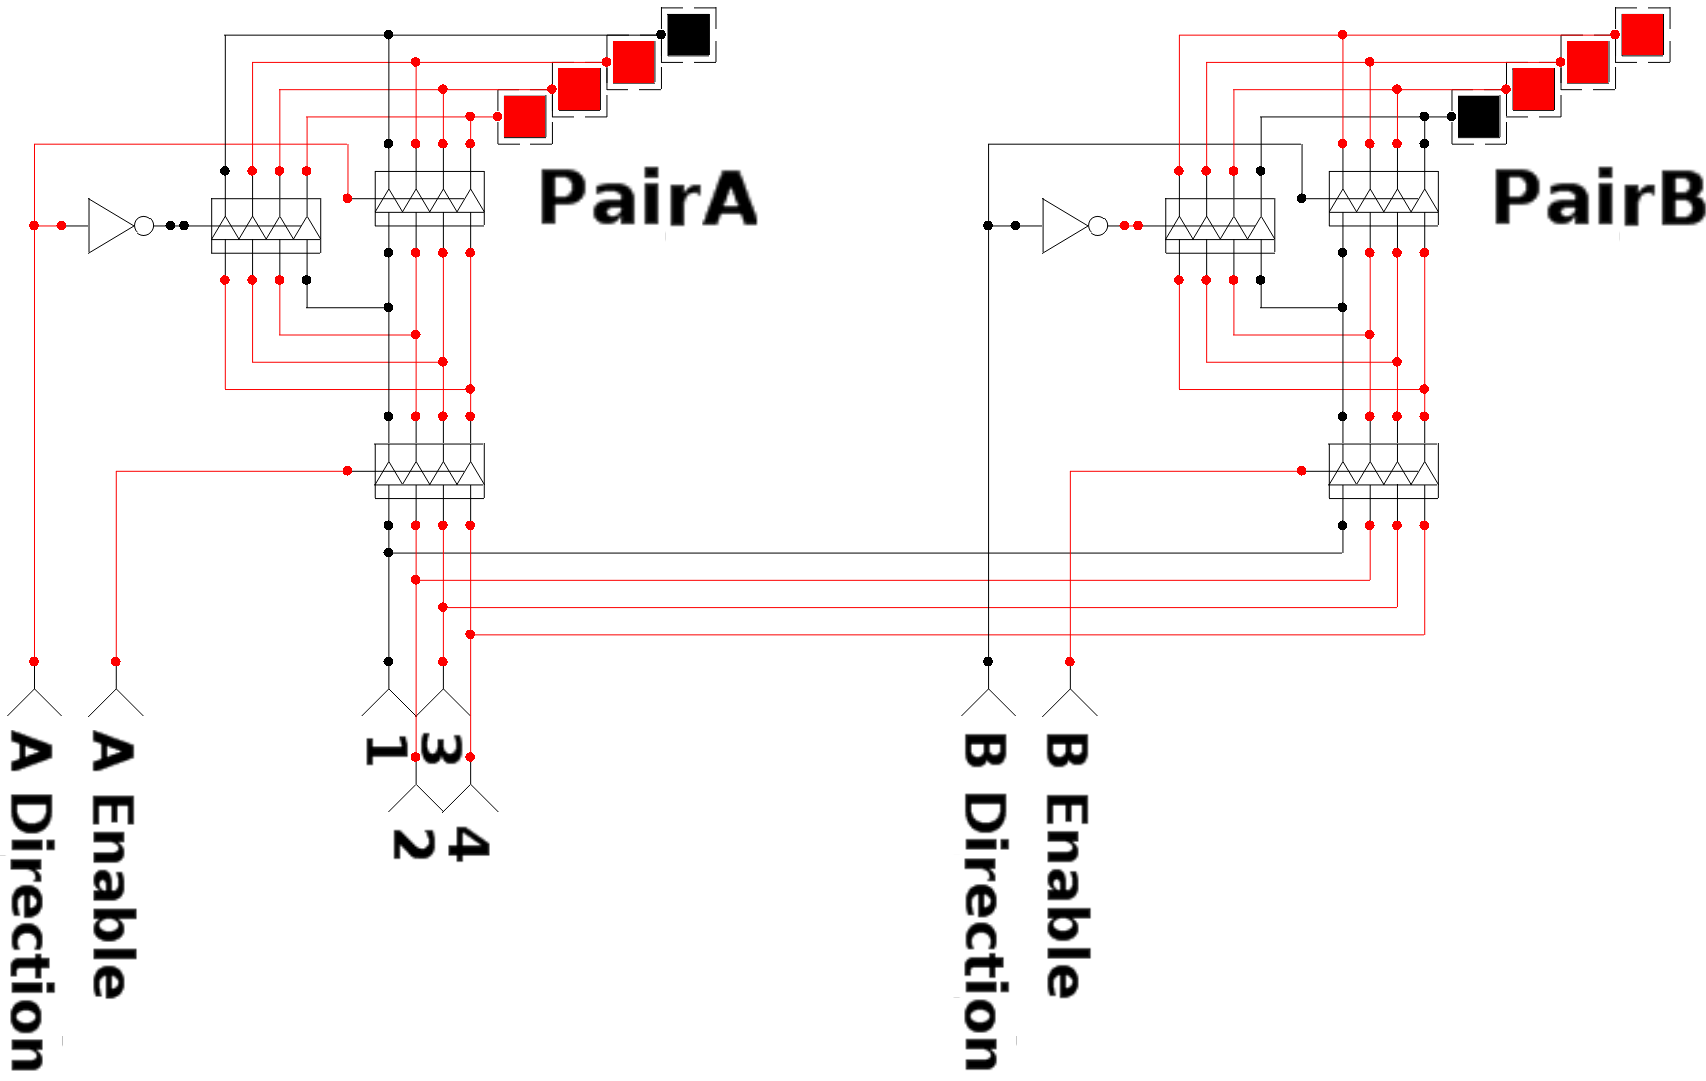
\includegraphics[width=0.2\textwidth]{figures/move/direction_choice}
	\caption{motor control circuit}
	\label{fig:mot_ctrl}
\end{figure}
%\missingfigure{schematic of motor control circuit}

We decided to use 6 tri-state buffers as shown in figure\ref{fig:mot_ctrl}.
